% Created: Enze Chen, June 2017

% Chapter 5 of the MSE 142 coursereader. 
% This chapter discusses the Kronig-Penney model for periodic potential barriers. 
% It doesn't delve too deep into the math behind Bloch wavefunctions, but just applies the result to calculate allowed energies. 
% This is a good model for electron transport through a solid and we will apply to result to look at electronic band structure.

% Uncomment the following three lines and last line to individually compile this chapter
%\documentclass[12pt, english]{book}
%\usepackage{142crstyle}
%\begin{document}

\chapter{Periodic Potentials} \label{ch:period}
%{ \doublespacing 
In the last chapter, we looked at quantum tunneling through a finite potential barrier, and we argued that the wavefunction and its first derivative must remain continuous even at discontinuities in the potential. 
What happens then, if the potential barrier at the discontinuity becomes infinitely tall yet infinitesimally narrow, like a huge needle? 
We will see in this chapter how this changes our continuity condition and how quantum tunneling allows us to use this new model to understand the transport properties of materials.


% % % % % % % % % % % % % % % % % % % % % % % % % % % % % % % % % % % % % 
% % % % % % % % % % % % % % % % % % % % % % % % % % % % % % % % % % % % % 
% % % % % % % % % % % % % % % % % % % % % % % % % % % % % % % % % % % % % 
\section{Before you begin}

This chapter builds on the following concepts, some of which we've already discussed in class, others you will likely have encountered elsewhere.
Mastery of these concepts will allow you to get the most out of this chapter.

\begin{itemize}
	\item Solving systems of equations.
	In a previous chapter we used the substitution method to solve a system, but here there will be a key step that uses some fundamental linear algebra properties to solve a homogeneous system (of the form $A \mathbf{x} = \mathbf{0}$).
	\begin{itemize}
		\item For additional details and practice, see \href{https://textbooks.math.gatech.edu/ila/solution-sets.html}{Georgia Tech} and \href{https://www.cuemath.com/algebra/homogeneous-system-of-linear-equations/}{Cuemath}.
	\end{itemize}

	\item Trigonometry, perhaps more specifically the cosine function.
	Know its roots, domain and range, and its relationship to the complex exponential function $e^{ix}$.
\end{itemize}

\begin{tcolorbox}[colframe=PaloAlto, colbacktitle=PaloAlto!20!white, title=Self-check quiz]
	We strongly recommend everyone to take \href{https://forms.gle/n5kDHJ5TQud5K9UZA}{the autograded quiz} for this chapter \emph{before} you begin.
	It is anonymous and doesn't affect your grade, but it will give you some feedback and situate you for what's about to come.
\end{tcolorbox}


% % % % % % % % % % % % % % % % % % % % % % % % % % % % % % % % % % % % % 
% % % % % % % % % % % % % % % % % % % % % % % % % % % % % % % % % % % % % 
% % % % % % % % % % % % % % % % % % % % % % % % % % % % % % % % % % % % % 
\section{Electron behavior}

We will start by providing a little more context around the problem at hand. 
In chemistry class, you might have learned that in metals, the electrons are spread out in a ``sea of electrons" and move around freely, which give metals good thermal and electrical conductivity. 
This effect, however, is in fact quite surprising. 
After all, there is a scattering center (atomic nucleus) every few angstroms in a solid---how do the electrons sneak by? 
We'll see how tunneling provides an answer that allows us to better understand electron transport and the band structure of materials. 

\begin{figure}[!h]
	\centering
	\includegraphics[width=0.5\linewidth]{comb.pdf}
	\caption{A schematic of the Kronig-Penney model that consists of an infinite periodic array of delta functions. 
	The potential is zero everywhere except at the delta functions, where it has a strength $g$.}
	\label{fig:comb}
\end{figure}

As with every chapter, we start by considering a representative toy model, which in this case consists of an infinite series of periodic \textbf{delta functions} spaced a distance $d$ apart (\autoref{fig:comb}). 
The question is how to solve for the wavefunction of an electron of total energy $E$ consistent with our requirement that the probability density function remains finite. 
This problem was first solved by Ralph Kronig and William Penney in 1931,\footnote{See R. Kronig and W. G. Penney, \href{http://rspa.royalsocietypublishing.org/content/130/814/499}{\emph{Proc. Roy. Soc. A}} 130, 1931. Their original formulation consisted of periodic rectangular blocks, while we jump straight to the typical approximation of height $\rightarrow\infty$ and width $\rightarrow0$.} so it is also known as the \textbf{Kronig-Penney model}.

The Kronig-Penney model is a good approximation for a crystal lattice, where the nuclei are periodic sites of infinite potential\footnote{OK, perhaps these should technically approach $-\infty$ to model attraction, but this way the math is cleaner.} and we assume zero potential everywhere else inside the lattice. 
To put this in mathematical terms, we can assign a periodicity to the potential such that 

\begin{equation*}
	V(x) = V(x+d)
\end{equation*}

In fact, we can go one step further and say that, given a potential strength of $g$, the series of potentials can be expressed as an infinite summation:

\begin{tcolorbox}[title = Kronig-Penney model potential] \vspace{-2ex}
	\begin{equation}
	V(x) = g \sum_{n=-\infty}^{\infty} \delta(x - nd) \label{eq:kp-pot}
	\end{equation}
\end{tcolorbox}

\noindent where $\delta(y)$ is the \textbf{Dirac delta function} given by

\begin{equation*}
	\boxed{\delta(y) = \begin{cases}
		+\infty & y=0 \\ 
		0 & y \neq 0
	\end{cases} \quad \text{ and } \quad 
	\int_{-\infty}^{\infty} \delta(y) \dd{y} = 1}
\end{equation*}


% % % % % % % % % % % % % % % % % % % % % % % % % % % % % % % % % % % % % 
% % % % % % % % % % % % % % % % % % % % % % % % % % % % % % % % % % % % % 
% % % % % % % % % % % % % % % % % % % % % % % % % % % % % % % % % % % % % 
\section{Bloch waves}

Now, since the electron behaves like a free particle between the delta functions, we know that its wavefunctions look like $\psi_n(x) = Ae^{ik_nx}$. 
This means that the electron density for a regular free particle, which is proportional to $\abs{\psi(x)}^2$, is a constant value. 
However, a constant isn't quite the correct solution here because then the translational invariance of the probability density function would be broken by the infinite potentials. 
To resolve this issue, we will instead argue that due to the periodicity of the lattice, it must be the case that the probability density function is also periodic, i.e. 

\begin{equation}
	\boxed{\abs{\psi(x)}^2 = \abs{\psi(x+d)}^2} \label{kp-period}
\end{equation}

In other words, if we know the probability density at one point $x$, since the potential is infinitely long and periodic (assume we are in the bulk solid and away from interfaces), this means we also know the probability density at $x+d$, $x+2d$, and so on. 
Now, what does this imply about the wavefunction itself? 
We can guess that the wavefunction is also periodic, at least up to a phase factor $e^{iqx}$ (this complex number will disappear when you take the modulus squared). 
This fact was formally proved in 1928 by Felix Bloch to describe the wavefunction of electrons in a crystalline lattice,\footnote{His \href{https://link.springer.com/article/10.1007\%2FBF01339455}{original paper} is in German, but \href{https://en.wikipedia.org/wiki/Bloch_wave}{Wikipedia} also gives a good explanation and even presents a proof.} and \textbf{Bloch's theorem} allows us to write the wavefunction as

\begin{tcolorbox}[title = Bloch wave equation] \vspace{-2ex}
	\begin{equation}
		\psi(x) = u(x)e^{iqx} \label{eq:bloch}
	\end{equation}	
\end{tcolorbox}

\noindent where the function $u(x)$ is periodic in $d$, i.e. $u(x) = u(x+d)$. 
To verify that this is a valid solution for the wavefunction, we can check to see if it satisfies \autoref{kp-period}.

\begin{align*}
	\psi(x+d) &= u(x+d)e^{iq(x+d)} \\
	\psi(x+d) &= u(x)e^{iqx}e^{iqd} \\
	\psi(x+d) &= \psi(x)e^{iqd} \numberthis \label{eq:bloch2}  \\
	\abs{\psi(x+d)}^2 &= \abs{\psi(x)}^2
\end{align*}

\noindent which is what we desired. 
The steps above are the key to the whole problem. 
Instead of trying to solve for the wavefunctions for all $x$, we only need to solve the \Sch\ equation in one period (from $x = 0$ to $x = d$, for example). 
Once we know the wavefunction there, we know it everywhere else by Bloch's theorem. 
What we claim is that the wavefunction for an electron in a periodic potential differs only from the wavefunction for a free particle by a periodic modulation, the function $u(x)$. 
This is quite remarkable! 
In the following sections we'll see how the variable $q$ really acts like a quantum number just as the integer $n$ did in the case of the particle in a box, where only certain ranges of $q$ will ultimately correspond to wave-like solutions.


% % % % % % % % % % % % % % % % % % % % % % % % % % % % % % % % % % % % % 
% % % % % % % % % % % % % % % % % % % % % % % % % % % % % % % % % % % % % 
% % % % % % % % % % % % % % % % % % % % % % % % % % % % % % % % % % % % % 
\section{Continuity condition}

We will start by designating the region $x \in (-d, 0)$ in \autoref{fig:comb} as $L$ and the region $x \in (0, d)$ as $R$. 
Each of these regions has zero potential, so the electron behaves as a free particle in these regions. 
We can then say that for $x \in (0, d)$, the electron has wavefunction solutions of the form 

\begin{equation}
	\psi_R(x) = A\sin(kx) + B\cos(kx) \label{eq:kpr}
\end{equation}

\noindent where $k = \sqrt{2mE/\hbar^2}$.

What about region $L$? 
In our derivation above, we observed in \autoref{eq:bloch2} that the wavefunction in adjacent regions differed only by a phase factor. 
We can rearrange that equation to obtain

\begin{equation}
	\psi(x) = e^{-iqd}\psi(x+d) \label{eq:bloch3}
\end{equation}

Aha! It might not be clear at first, but \autoref{eq:bloch3} allows us to express the wavefunction in region $L$ using the expression for the wavefunction in region $R$. 
Otherwise, we would have to use extra coefficients like $C$ and $D$ when writing down the wavefunction, which would complicate the math. 
Instead, we can say that for $x \in (-d,0)$, 

\begin{equation}
	\psi_L(x) = e^{-iqd}\left[A\sin(k(x+d)) + B\cos(k(x+d))\right] \label{eq:kpl}
\end{equation}

We need one more step to finish setting up our calculations, and that is the behavior of the wavefunction at $x = 0$ where the potential is discontinuous. 
We derived a continuity condition in the last chapter, but that was only under the assumption that the potential did not go to infinity, which is unfortunately not the case here. 
Instead, we will assume that the time-independent \Sch\ equation at the delta function takes the form 

\begin{equation*}
	-\frac{\hbar^2}{2m} \psi''(x) + g\delta(x) \psi(x) = E\psi(x)
\end{equation*}

Same as before, we will now integrate this equation over an infinitesimal region $(-\epsilon,\epsilon)$ to obtain:

\begin{align*}
	\int_{-\epsilon}^{\epsilon} -\frac{\hbar^2}{2m}  \psi''(x) \dd{x} + \int_{-\epsilon}^{\epsilon} g\delta(x) \psi(x) \dd{x} &= \int_{-\epsilon}^{\epsilon} E\psi(x) \dd{x} \\
	-\frac{\hbar^2}{2m} \int_{-\epsilon}^{\epsilon} \psi''(x) \dd{x} + g \int_{-\epsilon}^{\epsilon} \delta(x) \psi(x) \dd{x} &= E \int_{-\epsilon}^{\epsilon} \psi(x) \dd{x} \\
	-\frac{\hbar^2}{2m} \left[ \psi'|_{\epsilon} - \psi'_{-\epsilon} \right] + g \psi(0) &= 0 \\
	-\frac{\hbar^2}{2m} \left[ \psi'|_{\epsilon} - \psi'_{-\epsilon} \right] &= -g \psi(0)
\end{align*}

\begin{tcolorbox}[title = Continuity across the delta function potential] \vspace{-2ex}
	\begin{equation}
	\dv{\Psi}{x} \bigg|_{\epsilon} - \dv{\Psi}{x} \bigg|_{-\epsilon} = \frac{2mg}{\hbar^2}\psi(0) \label{eq:kp-cont}
	\end{equation}
\end{tcolorbox}

We see there is now a \textbf{discontinuity} in the \emph{first derivative} of the wavefunction at $x = 0$, which came as a result of integrating the delta function.\footnote{To do this, we applied the result $\int\delta(x-a)f(x) \dd{x} = f(a)$, which is known as the ``selection property'' of the delta function. Since $\delta(x-a)$ is only defined at $x=a$, it picks out the value of $f(a)$ (in this case, $\psi(0)$).} 
It is important to realize that the wavefunction itself is still continuous at the boundary just like it always was (again, probability argument works well here), even if its first derivative isn't.


% % % % % % % % % % % % % % % % % % % % % % % % % % % % % % % % % % % % % 
% % % % % % % % % % % % % % % % % % % % % % % % % % % % % % % % % % % % % 
% % % % % % % % % % % % % % % % % % % % % % % % % % % % % % % % % % % % % 
\section{Forbidden energies}

Now we have all the pieces assembled for the calculations, so it's time to roll up our sleeves and get to work. 
We will start by using the continuity conditions to get expressions for $A$ and $B$ from \autoref{eq:kpr} and \ref{eq:kpl}, and then proceed to derive an expression for $q$, which is what we ultimately want. 
At $x = 0$, we have by the continuity of the wavefunction that

\begin{align*}
	\psi_R(0) &= \psi_L(0) \\
	A\sin(0) + B\cos(0) &= e^{-iqd}\left[A\sin(kd) + B\cos(kd)\right] \\
	Ae^{-iqd}\sin(kd) + B\left(e^{-iqd}\cos(kd) - 1\right) &= 0 \numberthis \label{eq:kpc1}
\end{align*}

Now for the first derivatives, we have

\begin{align*}
	\psi_R'(0) &= Ak\cos(kx) - Bk\sin(kx) = Ak \\
	\psi_L'(0) &= e^{-iqd}\left[Ak\cos(kd) - Bk\sin(kd)\right]
\end{align*}

\noindent which we can plug into \autoref{eq:kp-cont} to obtain

\begin{align*}
	\psi_R'(0) - \psi_L'(0) &= \frac{2mg}{\hbar^2}\psi(0) \\
	Ak - Ae^{-iqd}k\cos(kd) + Be^{-iqd}k\sin(kd) &= \frac{2mg}{\hbar^2}B \\
	A \left(k - e^{-iqd}k\cos(kd)\right) + B\left(e^{-iqd}k\sin(kd) - \frac{2mg}{\hbar^2} \right) &= 0 \numberthis \label{eq:kpc2}
\end{align*}

\autoref{eq:kpc1} and \ref{eq:kpc2} give us two equations and two variables ($A$ and $B$), which we know how to solve! 
Of course, these equations look extremely ugly to solve by the substitution method, so we will take a more clever approach that can directly solve for $q$. 

You may have learned in your math classes that one way to solve linear systems of equations is by constructing a matrix. 
We will do that here in the following manner:

\begin{align*}
	Ae^{-iqd}\sin(kd) + B\left(e^{-iqd}\cos(kd) - 1\right) &= 0 \\
	A \left(k - e^{-iqd}k\cos(kd)\right) + B\left(e^{-iqd}k\sin(kd) - \frac{2mg}{\hbar^2} \right) &= 0 \\
	\Downarrow \qquad \qquad \qquad \qquad & \\
	\underset{Q}{\underbrace{\begin{bmatrix}
		e^{-iqd}\sin(kd) & e^{-iqd}\cos(kd) - 1 \\ k\left(1 - e^{-iqd}\cos(kd)\right) & e^{-iqd}k\sin(kd) - \frac{2mg}{\hbar^2}
	\end{bmatrix}}} \begin{bmatrix}
		A \\ B
	\end{bmatrix} &= \begin{bmatrix}
		0 \\ 0
	\end{bmatrix}\numberthis \label{eq:kpmat}
\end{align*}

\noindent where we have a complicated coefficient matrix $Q$ multiplying our variables vector. 
We can see right away that a trivial solution to this equation is $A = B = 0$, which can't be the correct solution because it would lead to a degenerate wavefunction. 
Instead, we note that allowable solutions (of which there are infinitely many) to \autoref{eq:kpmat} are obtained when the determinant of $Q$ is zero.\footnote{This is discussed briefly on \href{https://en.wikipedia.org/wiki/System_of_linear_equations\#Homogeneous_systems}{Wikipedia}.} 
Calculating the determinant\footnote{For a $2\times2$ matrix $Q=\begin{pmatrix} a & b \\ c & d	\end{pmatrix}$, the determinant is given by $\det(Q) = ad - bc$.} and setting it equal to zero gives us an equation for $q$ that we can then solve. 
Proceeding, we find

\begin{align*}
	\det(Q) &= 0 \\
	e^{-iqd}\sin(kd) \left( e^{-iqd}k\sin(kd) - \frac{2mg}{\hbar^2} \right) &= \left( e^{-iqd}\cos(kd) - 1 \right) \left( k\left(1 - e^{-iqd}\cos(kd)\right) \right) \\
	ke^{-2iqd} \sin^2(kd) - \frac{2mg}{\hbar^2}e^{-iqd}\sin(kd) &= k\left[ e^{-iqd}\cos(kd) - e^{-2iqd}\cos^2(kd) - 1 + e^{-iqd}\cos(kd) \right]
\end{align*}

\noindent Now we multiply both sides by $e^{iqd}$.

\begin{align*}
	ke^{-iqd}\sin^2(kd) - \frac{2mg}{\hbar^2}\sin(kd) &= k\left[ \cos(kd) - e^{-iqd}\cos^2(kd) - e^{iqd} + \cos(kd) \right] \\
	ke^{-iqd}\sin^2(kd) + ke^{-iqd}\cos^2(kd) - \frac{2mg}{\hbar^2}\sin(kd) &= 2k\cos(kd) - ke^{iqd} \\
	ke^{-iqd} + ke^{iqd} - \frac{2mg}{\hbar^2}\sin(kd) &= 2k\cos(kd) \\
	k \left(2 \cdot \frac{e^{-iqd} + e^{iqd}}{2} \right) &= 2k\cos(kd) + \frac{2mg}{\hbar^2}\sin(kd)\\
	2k\cos(qd) &= 2k\cos(kd) + \frac{2mg}{\hbar^2}\sin(kd)
\end{align*}

We finish this off by dividing by $2k$ and multiplying the second term on the right hand side (RHS) by $\frac{d}{d}$ to create another $\frac{\sin(x)}{x}$ term. 
This gives us

\begin{tcolorbox}[title = Kronig-Penney model allowed solutions] \vspace{-2ex}
	\begin{equation}
		\cos(qd) = \cos(kd) + P\frac{\sin(kd)}{kd} \label{eq:kp}
	\end{equation}
\end{tcolorbox}

\noindent where $P = \dfrac{mgd}{\hbar^2}$.

To see what we can glean from this equation, the RHS of \autoref{eq:kp} is plotted as a function of $kd$ in \autoref{fig:kp}.

\begin{figure}[!h]
	\centering 
	\includegraphics[width=0.55\linewidth]{kp-rhs.pdf}
	\caption{A plot of the right hand side of \autoref{eq:kp} is shown in blue. 
	The hatched areas are forbidden values for $k$ (and hence, the energy) because they lie outside the range of cosine, and thus can never be equal to $\cos(qd)$ on the left hand side. 
	This leaves a series of energy bands of allowed electron states (orange).}
	\label{fig:kp}
\end{figure}

One observes immediately that there are ranges of $k$ and therefore ranges of $E$ (since $k = \sqrt{2mE/\hbar^2})$ for which no value of $k$ in that range satisfies \autoref{eq:kp}, as the curve oscillates outside the region between $-1$ and $1$. 
In particular, at low energies, there is a region for which there is no solution. 
This might be expected: For very small $E$ compared to the potential barrier, the electrons can't propagate through the periodic potential because the barriers are too high. 
At higher $E$, the curve enters the region between $[-1,1]$ corresponding to well-defined solutions. 
These resemble wave-like solutions of the form given by the Bloch wave equation (\autoref{eq:bloch}) and with $q$ specified by \autoref{eq:kp}. 
The lowest energy ground state is non-zero, consistent with the notion that the ground state energy always has value greater than the minimum value of the potential (we saw this similarly for the solution to the particle in a box). 
At higher energies, the curve again exits the region of allowed solutions, corresponding to a region for which propagating solutions do not exist. 
Remarkably, this corresponds to the existence of a band gap in the material, which we will show in the following section.


% % % % % % % % % % % % % % % % % % % % % % % % % % % % % % % % % % % % % 
% % % % % % % % % % % % % % % % % % % % % % % % % % % % % % % % % % % % % 
% % % % % % % % % % % % % % % % % % % % % % % % % % % % % % % % % % % % % 
\section{Application: Band structure}

Recall that our original motivation for the Kronig-Penney model was to model the behavior of electrons inside a material. 
Due to the presence of periodically-spaced atomic nuclei that act as scattering centers, such as in a crystal lattice, the wave-like electrons cannot have arbitrary energies. 
Instead, they are confined to \textbf{bands} of energy and forbidden from other regions; together, these bands and regions constitute the \textbf{band structure} of a material and are fundamental to the optical and electronic properties of a material. 

In order to calculate the band structure, we look to \autoref{eq:kp}. 
To better see the relationship between the LHS and RHS, we have plotted a close-up of the first energy band in \autoref{fig:kp-zoom}. 
At point $A$, the RHS equals 1, which leads to

\begin{equation*}
	\cos(qd) = 1 \implies q = 0
\end{equation*}

\begin{figure}[!h]
	\centering 
	\includegraphics[width=0.55\linewidth]{kp-rhs-zoom.pdf}
	\caption{A close-up of the first energy band shown in \autoref{fig:kp}. 
	The labeled points demonstrate clear correspondences between $q$ and $k$.}
	\label{fig:kp-zoom}
\end{figure}

We can do the same with the other three points, and we consolidate the results in \autoref{tab:qvk}.

\begin{table}[!h]
	\centering
	\begin{tabular}{crlc}
		Point & RHS & Equation & $q$ \\ \toprule
		$A$ & 1 & $\cos(qd) = 1$ & 0 \\
		$B$ & 0 & $\cos(qd) = 0$ & $\pi/2d$ \\
		$C$ & $-1$ & $\cos(qd) = -1$ & $\pi/d$ \\
		$D$ & $-1$ & $\cos(qd) = -1$ & $\pi/d$
	\end{tabular}
	\caption{Four correspondence points near the first energy band that show the relationship between $q$ and $k$.}
	\label{tab:qvk}
\end{table}

Note that at point $A$, $q = 0$ corresponds to a non-zero value of $k$ and hence a non-zero value for the energy, which we have previously discussed. 
Also, even though $q = \pi/d$ at both $C$ and $D$, those points are at different energy levels. 
This means if we construct a plot of $E$ vs. $q$, as we have done in \autoref{fig:Evq}, we will see a jump discontinuity at $q = \pi/d$---and thus the band gap emerges! 
This pattern continues at every multiple of $\pi/d$, and the width of each successive energy band increases while the gap in between them slowly decreases. 
Instead of having discrete energy levels like in the particle in a box model, here the energies have spread out into wider bands due to quantum interactions between neighboring wavefunctions across the potential barrier.

\begin{figure}[!h]
	\centering
	\subfloat[]{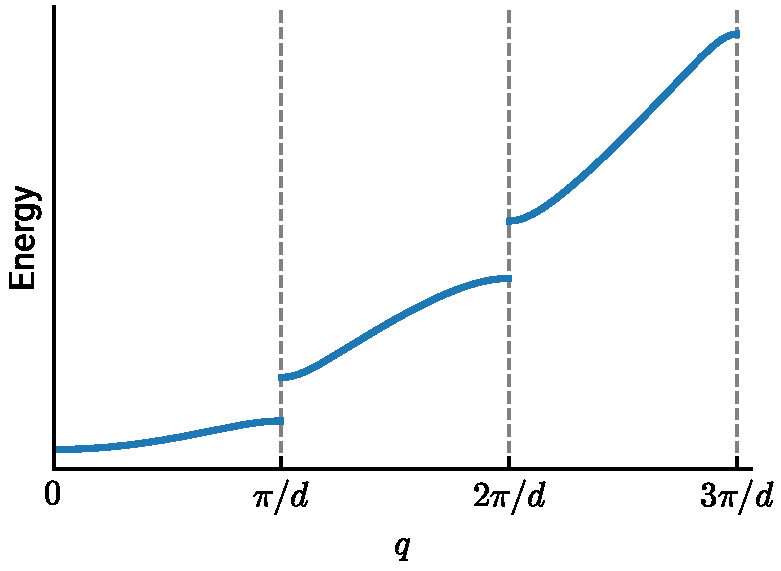
\includegraphics[width=0.49\linewidth]{E-vs-q-1.pdf} \label{fig:Evq1}}
	\hfill
	\subfloat[]{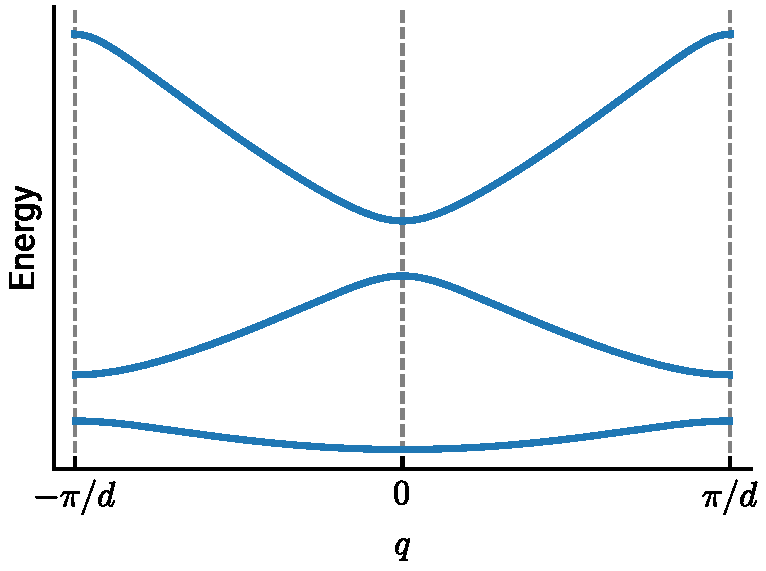
\includegraphics[width=0.49\linewidth]{E-vs-q-2.pdf} \label{fig:Evq2}}
	\caption{A plot of $E$ vs. $q$ in \protect\subref{fig:Evq1} expanded form and 
	\protect\subref{fig:Evq2} reduced form, where we have translated the energy bands to fit within the first Brillouin zone.}
	\label{fig:Evq}
\end{figure}

Now, in a class like ENGR 50 or MATSCI 143, you have used a unit cell to characterize many of the properties of the bulk crystal. 
It turns out there's a direct analogy here thanks to the Bloch wave description we saw earlier. 
Instead of drawing out the energy bands in an expanded form like we did in \autoref{fig:Evq1}, we will first translate each band by a multiple of $2\pi/d$ until it lies within the interval from $[-\pi/d, \pi/d]$. 
We then take that image and reflect it across the $y$-axis to produce the symmetric image shown in \autoref{fig:Evq2}. 
This region from $[-\pi/d, \pi/d]$ is called the \textbf{first Brillouin zone} (pronounced ``Bree-luwan'') and it is sufficient to characterize all of the wave vectors of the electron moving through a periodic potential. 
You can think of it as the unit cell equivalent in momentum space, or what's more commonly known as \textbf{reciprocal space}. 
These fascinating topics are unfortunately outside the scope of this course, but I encourage you to do some research on your own as they build beautifully on top of what we've seen so far.

OK, now that we've shown the existence of the band gap within a material's band structure, why should we \emph{care}? 
Well, we've already stated that inside the band gap, no electronic states can exist. 
This means that electrons must exist in the band right below it, known as the \textbf{valence band}, or acquire enough energy to be promoted to the upper energy band, known as the \textbf{conduction band}. 
It turns out that only electrons in the conduction band are free to move within the crystal lattice and conduct electric current, so right away we can see how the band gap determines whether a material is a metal, semiconductor, or insulator (\autoref{fig:bgs}).

\begin{figure}[!h]
	\centering
	\includegraphics[width=0.7\linewidth]{bandgaps.pdf}
	\caption{Schematic of the different band structures in metals, semiconductors, and insulators.}
	\label{fig:bgs}
\end{figure}

Typically, the two energy bands in a metal overlap, which give metals good conductivity since there is no band gap to overcome! 
On the other hand, the bands are so far apart in insulators that it becomes impossible for electrons to gain enough energy to overcome the band gap and conduct electricity. 
Semiconductors are a hot topic of research precisely due to their small band gap that can be tuned to modulate the amount of energy it takes for electrons to cross the barrier. 
Band gap engineering typically involves changing a material's chemical composition, stress state, layer thickness, and/or morphological patterning to control the positions of the energy bands, which has led to huge advancements in solar cells,\footnote{Featuring Michael McGehee, a former Stanford MSE professor. See E. T. Hoke et al. \href{https://pubs.rsc.org/en/content/articlelanding/2015/sc/c4sc03141e}{\emph{Chem. Sci.}} 6, 2015 and G. E. Eperon et al. \href{http://science.sciencemag.org/content/354/6314/861.full}{\emph{Science}} 354, 2016.} optoelectronics,\footnote{Featuring Mark Brongersma from our MSE department. See D. S. Sukhdeo et al. \href{https://www.osapublishing.org/oe/abstract.cfm?uri=oe-23-13-16740}{\emph{Optics Express}} 23, 2015.} and photonics.\footnote{Featuring Shanhui Fan from Stanford's EE department. See J. D. Joannopoulos et al. \href{https://www.nature.com/articles/386143a0}{\emph{Nature}} 386, 1997. This article, albeit a little dated, gives a thorough introduction into the analogous \emph{photonic} band gap.}


% % % % % % % % % % % % % % % % % % % % % % % % % % % % % % % % % % % % % 
% % % % % % % % % % % % % % % % % % % % % % % % % % % % % % % % % % % % % 
% % % % % % % % % % % % % % % % % % % % % % % % % % % % % % % % % % % % % 
\section{Summary}

To recap, this chapter exposed us to the idea of a periodic potential modeled as a series of delta functions in the Kronig-Penney model. 
We applied Bloch's theorem to describe the periodicity in an electron's wavefunction and derive a new continuity condition across the potential barriers. 
This allowed us to derive an equation for the relationship between the phase shift wave number $q$ and the electron's energy $E$. 
We discovered that the result was a good model for the band structure of a material, and that there were certain regions of energy that were forbidden for the electron, thus demonstrating the existence of a material's band gap. 
The Kronig-Penney model's simplistic nature and uncanny ability to elucidate the band gap make it a powerful model for periodic quantum mechanical systems. 

So far, all of the potentials we've encountered have been rectangular, although this need not be the case. 
Coming up next, we will explore the behavior of particles in a parabolic potential, which describes simple harmonic motion in a quantum mechanical system. 
Get ready to work with some of the nifty mathematical tools contained within quantum theory!

%} % for doublespacing
%\end{document}